\documentclass{report}
\usepackage[utf8]{inputenc}
\usepackage{hyperref}
\usepackage{graphicx}
\usepackage{float}
\usepackage{caption}
\usepackage{subcaption}

\title{Group Project Report:\\Robin}
\author{Robert Bastian\\Paavan Buddhdev\\Aiken Cairncross\\James Dai\\Alistair Gavin\\\\\\Supervisor: Ivo Sluganovic\\Corporate Sponsor: \emph{Palantir}\\\\University of Oxford}
\date{May 2015}

\begin{document}

\maketitle
\tableofcontents

\chapter{Specification and planning}
In this section we will outline the brief we were given, our initial ideas for what project to do, a flow-diagram for our chosen idea, and our plan of action. At the end, a full project specification is included. Full details about the implementation will be covered in the second half of this report.

\section{The brief}
The following was the brief that we selected from the list of possible projects:

\begin{quote}Project K: Gamification\\There have been many attempts to improve the way that key skills are developed throughout a programmer's career, and one of the ways that has proven to be highly effective is gamification. When done correctly, gamification can provide motivation to learn new skills, or hone existing ones. The challenge is to create a group game that develops one or more core skills that you consider to be important to programmers. The game can be collaborative or competitive, but it must be easy to set up and most importantly fun. If you have an awesome idea that requires a little hardware, Palantir will happily cover any reasonable costs.\\Example project: "Security Capture the Flag". Write a web server with typical security vulnerabilities and install it on a Raspberry Pi. Players compete against each other to gain the most complete control of the Pi in the fastest time. In this example, real time competition provides an extra incentive for players to do well (a common example of gamification). Global leaderboards and bonuses for completing optional challenges can also motivate players, and reward players for focusing efforts towards a particular skill (for example, providing a bonus for responding to a new defence within a time limit, to encourage players to write maintainable, extendable code).\end{quote}

\section{Our initial ideas}
From this brief, we had a lot of ideas coming out of our initial discussions
\begin{description}
\item[‘Kevin’ / Minigames] \hfill \\ The player controls a character travelling through a 2D world, whose progress is
determined by the player solving simple programming challenges that are encountered by Kevin within different minigames. Optional paths are also available, so that players of different skill levels are also challenged.
\item[Digital systems game] \hfill \\The player builds logic circuits to solve progressively more difficult challenges. At each level the player has access to components that had previously been built, which helps to teach different layers of abstractions.
\item['Extreme startup' style game] \hfill \\The players would write software to interpret and reply to requests from a central server. The system would award points to each player for every correct response, and deduct for incorrect responses or errors.
\item[Classroom Pi] \hfill \\The users learn basic programming concepts (for loops, conditional statements, etc.) by programming on a Raspberry Pi. This idea was intended to be used in a classroom environment, where the students would learn the different concepts while working in teams / small groups, whilst within a supervised environment.
\item['The Elevator Game'] \hfill \\The player programs one or more elevators. The elevators are required to transport a certain number of people to the floor they each want to go to in the quickest time possible. Each successive level increases in complexity, e.g. more people, fewer elevators, stricter weight restrictions, etc.
\item[The round-robin challenge] \hfill \\Teams of players create challenges for each other to solve within a limited time-frame. After the expiry date, the challenge setter rates each of the solutions, and the other players rate the challenge. A new challenge is then chosen, and the game moves on in a round-robin format. The challenges are language-independent.
\end{description}


\section{Our chosen idea (and the reasons why we chose it)}
Our chosen idea was the round-robin challenge system. We had three main reasons for choosing it, as opposed to the other ideas:
\begin{enumerate}
\item The other ideas, while all involving the user playing a game, were not as directly focused on \textbf{competitiveness} - any competition was implemented by using high scores and best times. The round-robin idea involved directly challenging other players, which we think is the best way to keep people interested and motivated and thus the best way for users to learn more about programming.
\item By leaving the details of challenges up to the players, there was a lot of \textbf{scope} for players to go where they wanted. Teams of experienced developers have the ability set more difficult challenges for each other.
\item Moreover, implementing this idea of a \textbf{`metagame`} allowed us to focus on building a framework for setting challenges for different users using a server instead of getting bogged down in specific details, which was something we were all keen to try out.
\end{enumerate}
While the idea may initially seem quite simple, we were wary of being too ambitious, as few of us had worked on a project like this before.

\section{Proposed lifecycle of a challenge}
The following diagram was our conceptual run-through of how one round of our round-robin tournament would go. In this diagram the actors are underlined, and any potential ideas, advanced features or undecided design decisions are italicized.

\begin{enumerate}
\item While no challenge is active, the \underline{players} can submit a challenge
\begin{itemize}
\item Each challenge comprises
\begin{itemize}
\item Title, description, sample dataset / sample input
\item A grading method
\begin{itemize}
\item By default the \underline{Question Master} grades each solution
\item \emph{Or could be automatically graded? Or the solvers grade (peer reviewed)}
\end{itemize}
\item Expiry date
\end{itemize}
\item \emph{Can challenge be changed if a problem is found with it? How is this dealt with?}
\item \emph{Should we allow a challenge be added to the queue whenever or only when none active?}
\end{itemize}
\item A \underline{Question Master} is chosen
\begin{itemize}
\item The Question Master has to be someone who has submitted a challenge.
\item \emph{Chosen in a round-robin order? Can \underline{users} choose to pass?}
\item Chosen based on points from last round / winner of last round?
\item \emph{Chosen by random allocation?}
\end{itemize}
\item Everyone else becomes a \underline{solver}. Each \underline{solver}:
\begin{itemize}
\item Gets a challenge and solves the challenge
\item \emph{Submits their solution as code? Or as text? Sent by email or through a web app or directly to a server?}
\item \emph{A more advanced: allow solvers to modify or resubmit solutions}
\end{itemize}
\item \underline{Solvers} grade the challenge, and the \underline{question-master} grades the solutions
\begin{itemize}
\item Grading of challenge by submitters
\item \emph{A more advanced way would grade by combining ratings in the categories
\begin{itemize}
\item Complexity
\item Ingenuity/technical
\item Fun factor
\end{itemize}}
\item Grading of solutions
\item \emph{If consensus is that challenge is bad (e.g. 40\% down-votes) then scrap challenge?}
\item \emph{Questions / challenges posed to challenger? Is this done irl or in the system?}
\end{itemize}
\item Points allocated to
\begin{itemize}
\item \underline{Solvers} and \underline{challengers}
\begin{itemize}
\item \emph{Include a bias to incentivise people to choose to set challenges – setting challenges gets more points / placed at top of board?}
\end{itemize}
\end{itemize}
\item Leaderboard updated with points of each participant
\item Challenge archived\\\\\\\\
\end{enumerate}

\section{Use cases}
The main use cases are outlined in Figures 1.1-1.4
{
\floatstyle{boxed}
\restylefloat{figure}

\begin{figure}[H]
\caption{Logging in}
\begin{description}
\item[Primary actor] Users
\item[Goal] To log in
\item[Main Success Scenario]~
\begin{enumerate}
\item The user enters their username and password
\item The server checks if the username is a correct username and that the password entered matches the user’s password
\item The user is logged in
\end{enumerate}
\item[Extensions] If the username or password is not correct, the server informs the user to retry
\end{description}
\end{figure}

\begin{figure}[H]
\caption{Setting a challenge}
\begin{description}
\item[Primary actor] Question Master
\item[Goal] To set a challenge for others to solve if none already is
\item[Stakeholders]~
\begin{enumerate}
\item Question Master: wants to set the challenge
\item Solvers: wants to have a challenge to solve
\end{enumerate}
\item[Trigger] a user gains the right to set a challenge
\item[Main Success Scenario]~
\begin{enumerate}
\item The QM decides on the challenge
\item The QM inputs the challenge into the web app and selects an end time
\end{enumerate}
\end{description}
\end{figure}

\begin{figure}[H]
\caption{Submitting a solution}
\begin{description}
\item[Primary actor] Solvers
\item[Goal] To submit a solution to the current challenge
\item[Stakeholders]~
\begin{enumerate}
\item Question Master: wants to have their challenge solved
\item Solvers: wants to solve the challenge
\end{enumerate}
\item[Success guarantees] The solution is submitted to the server
\item[Trigger] The QM sets a question
\item[Main Success Scenario]~
\begin{enumerate}
\item The solver reads the question and decides upon a solution
\item The solver types their solution and submits it
\end{enumerate}
\end{description}
\end{figure}

\begin{figure}[H]
\caption{Scoring}
\begin{description}
\item[Primary actor] Users
\item[Goal] To score the challenges and solutions
\item[Stakeholders]~
\begin{enumerate}
\item Question Master: wants to be able to rate solutions and have their challenge rated
\item Solvers: wants to rate the challenge and have their solutions rated
\end{enumerate}
\item[Success guarantees] Scores are submitted successfully
\item[Trigger] The current question expires
\item[Main Success Scenario]~
\begin{enumerate}
\item Each solver has to rate the challenge
\item The QM rates each individual solution
\end{enumerate}
\end{description}
\end{figure}
}

\clearpage

\section{Collaboration methods and group roles}
We decided to use \emph{Slack} as our main communication method. \emph{Slack} is a multi-platform program which allowed us to converse, and organise our conversations in different channels, each with a specific purpose. This allowed us to discuss the tasks that needed to be done separately, which different was really useful when working on separate modules of the application.

We used the \emph{Git} version control system to collaborate on the code. It was essential as it allowed us to keep working on the same project when not in the same place, which was especially important during the break, when we were all very far away from each other and had very different schedules.

After initially considering using \emph{Asana} to organise tasks, we decided that it would overcomplicate things, and that \emph{Slack} and \emph{Git} were sufficient for our needs.

\chapter{Design and Implementation}
After we had our specification and our plan, our next step was to implement the various components (e.g. the web interface, the Rails server, the structure for setting challenges, the structure for rating challenges and solutions, etc.). This second half of this report shall explain how we planned these components, and then integrated them together. It will also go over how we tested the system and the challenges we encountered.

\section{Design/layout mockups}
Figures 2.1-2.3 are some of the initial drawings from one of our first sessions for what the site structure will look like.

\begin{figure}[H]
\centerline{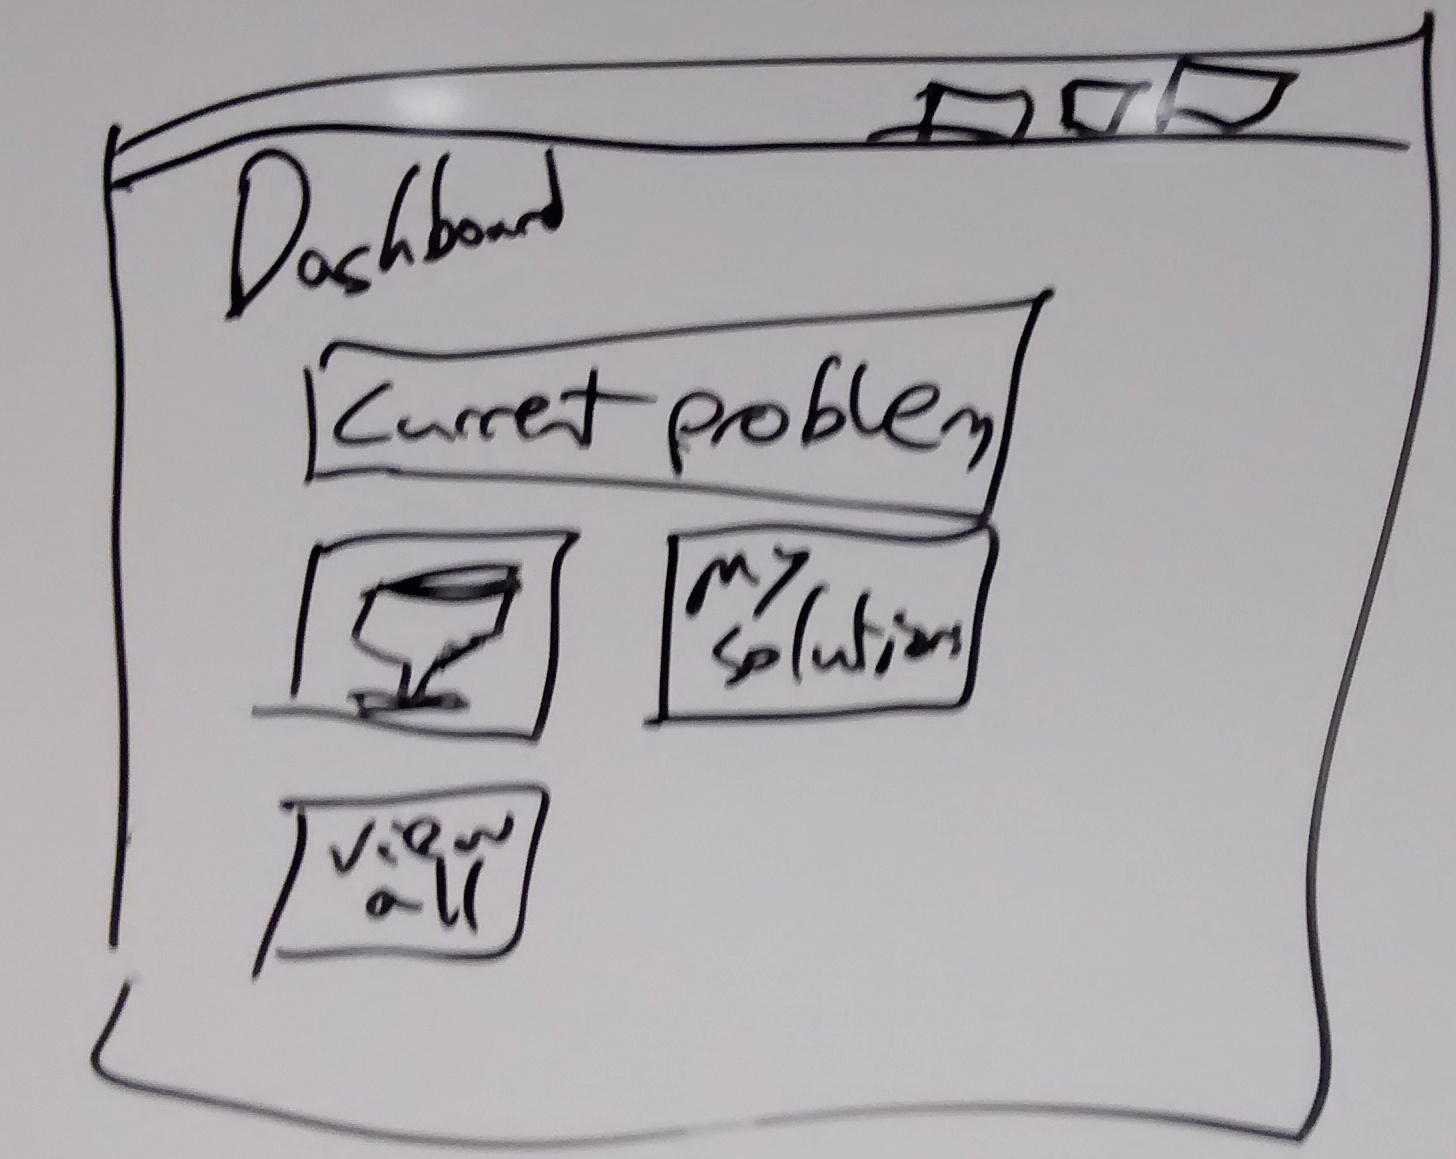
\includegraphics[height=6cm]{dashboardMockup}}
\caption{Dashboard}
\end{figure}

\begin{figure}[H]
\centerline{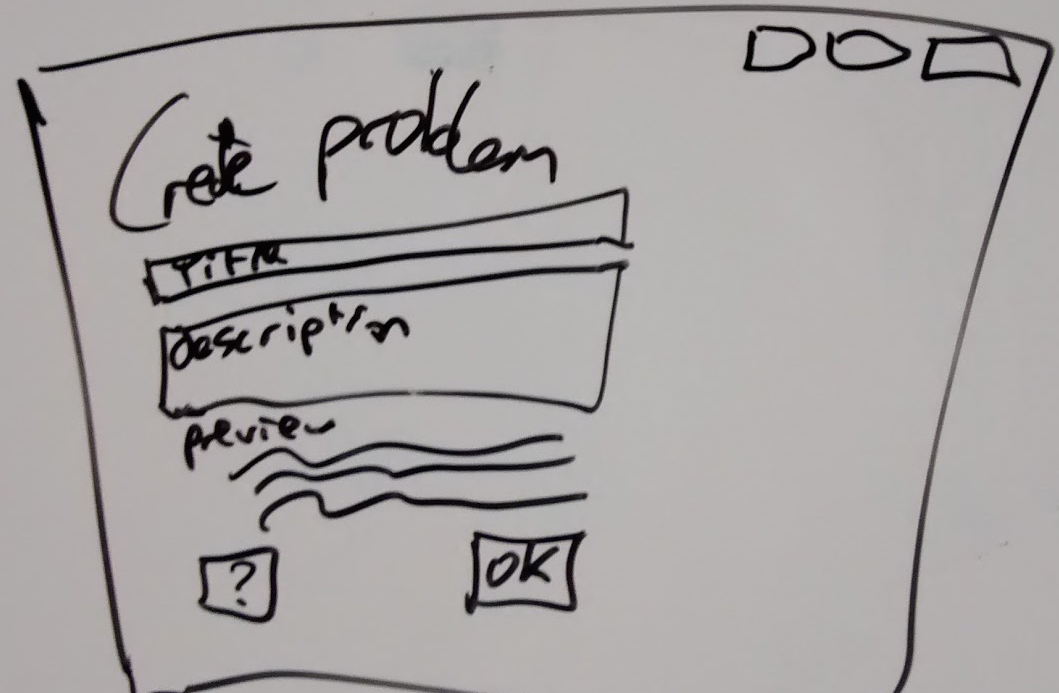
\includegraphics[height=6cm]{newProblemMockup}}
\caption{Challenge submission}
\end{figure}

\begin{figure}[H]
\centerline{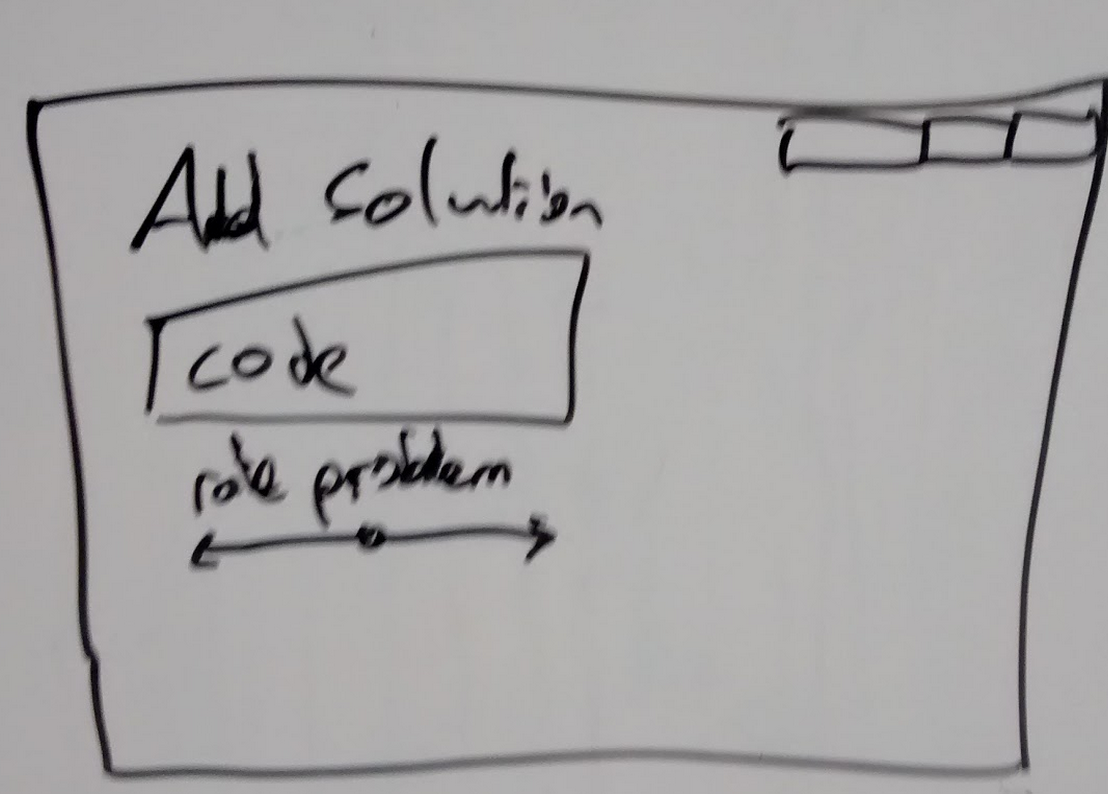
\includegraphics[height=6cm]{newSolutionMockup}}
\caption{Solution submission}
\end{figure}

\section{Site structure and state diagram}
Figures 2.4-2.6 are the initial outlines for the app’s database (model) and its website structure (views).

\begin{figure}[H]
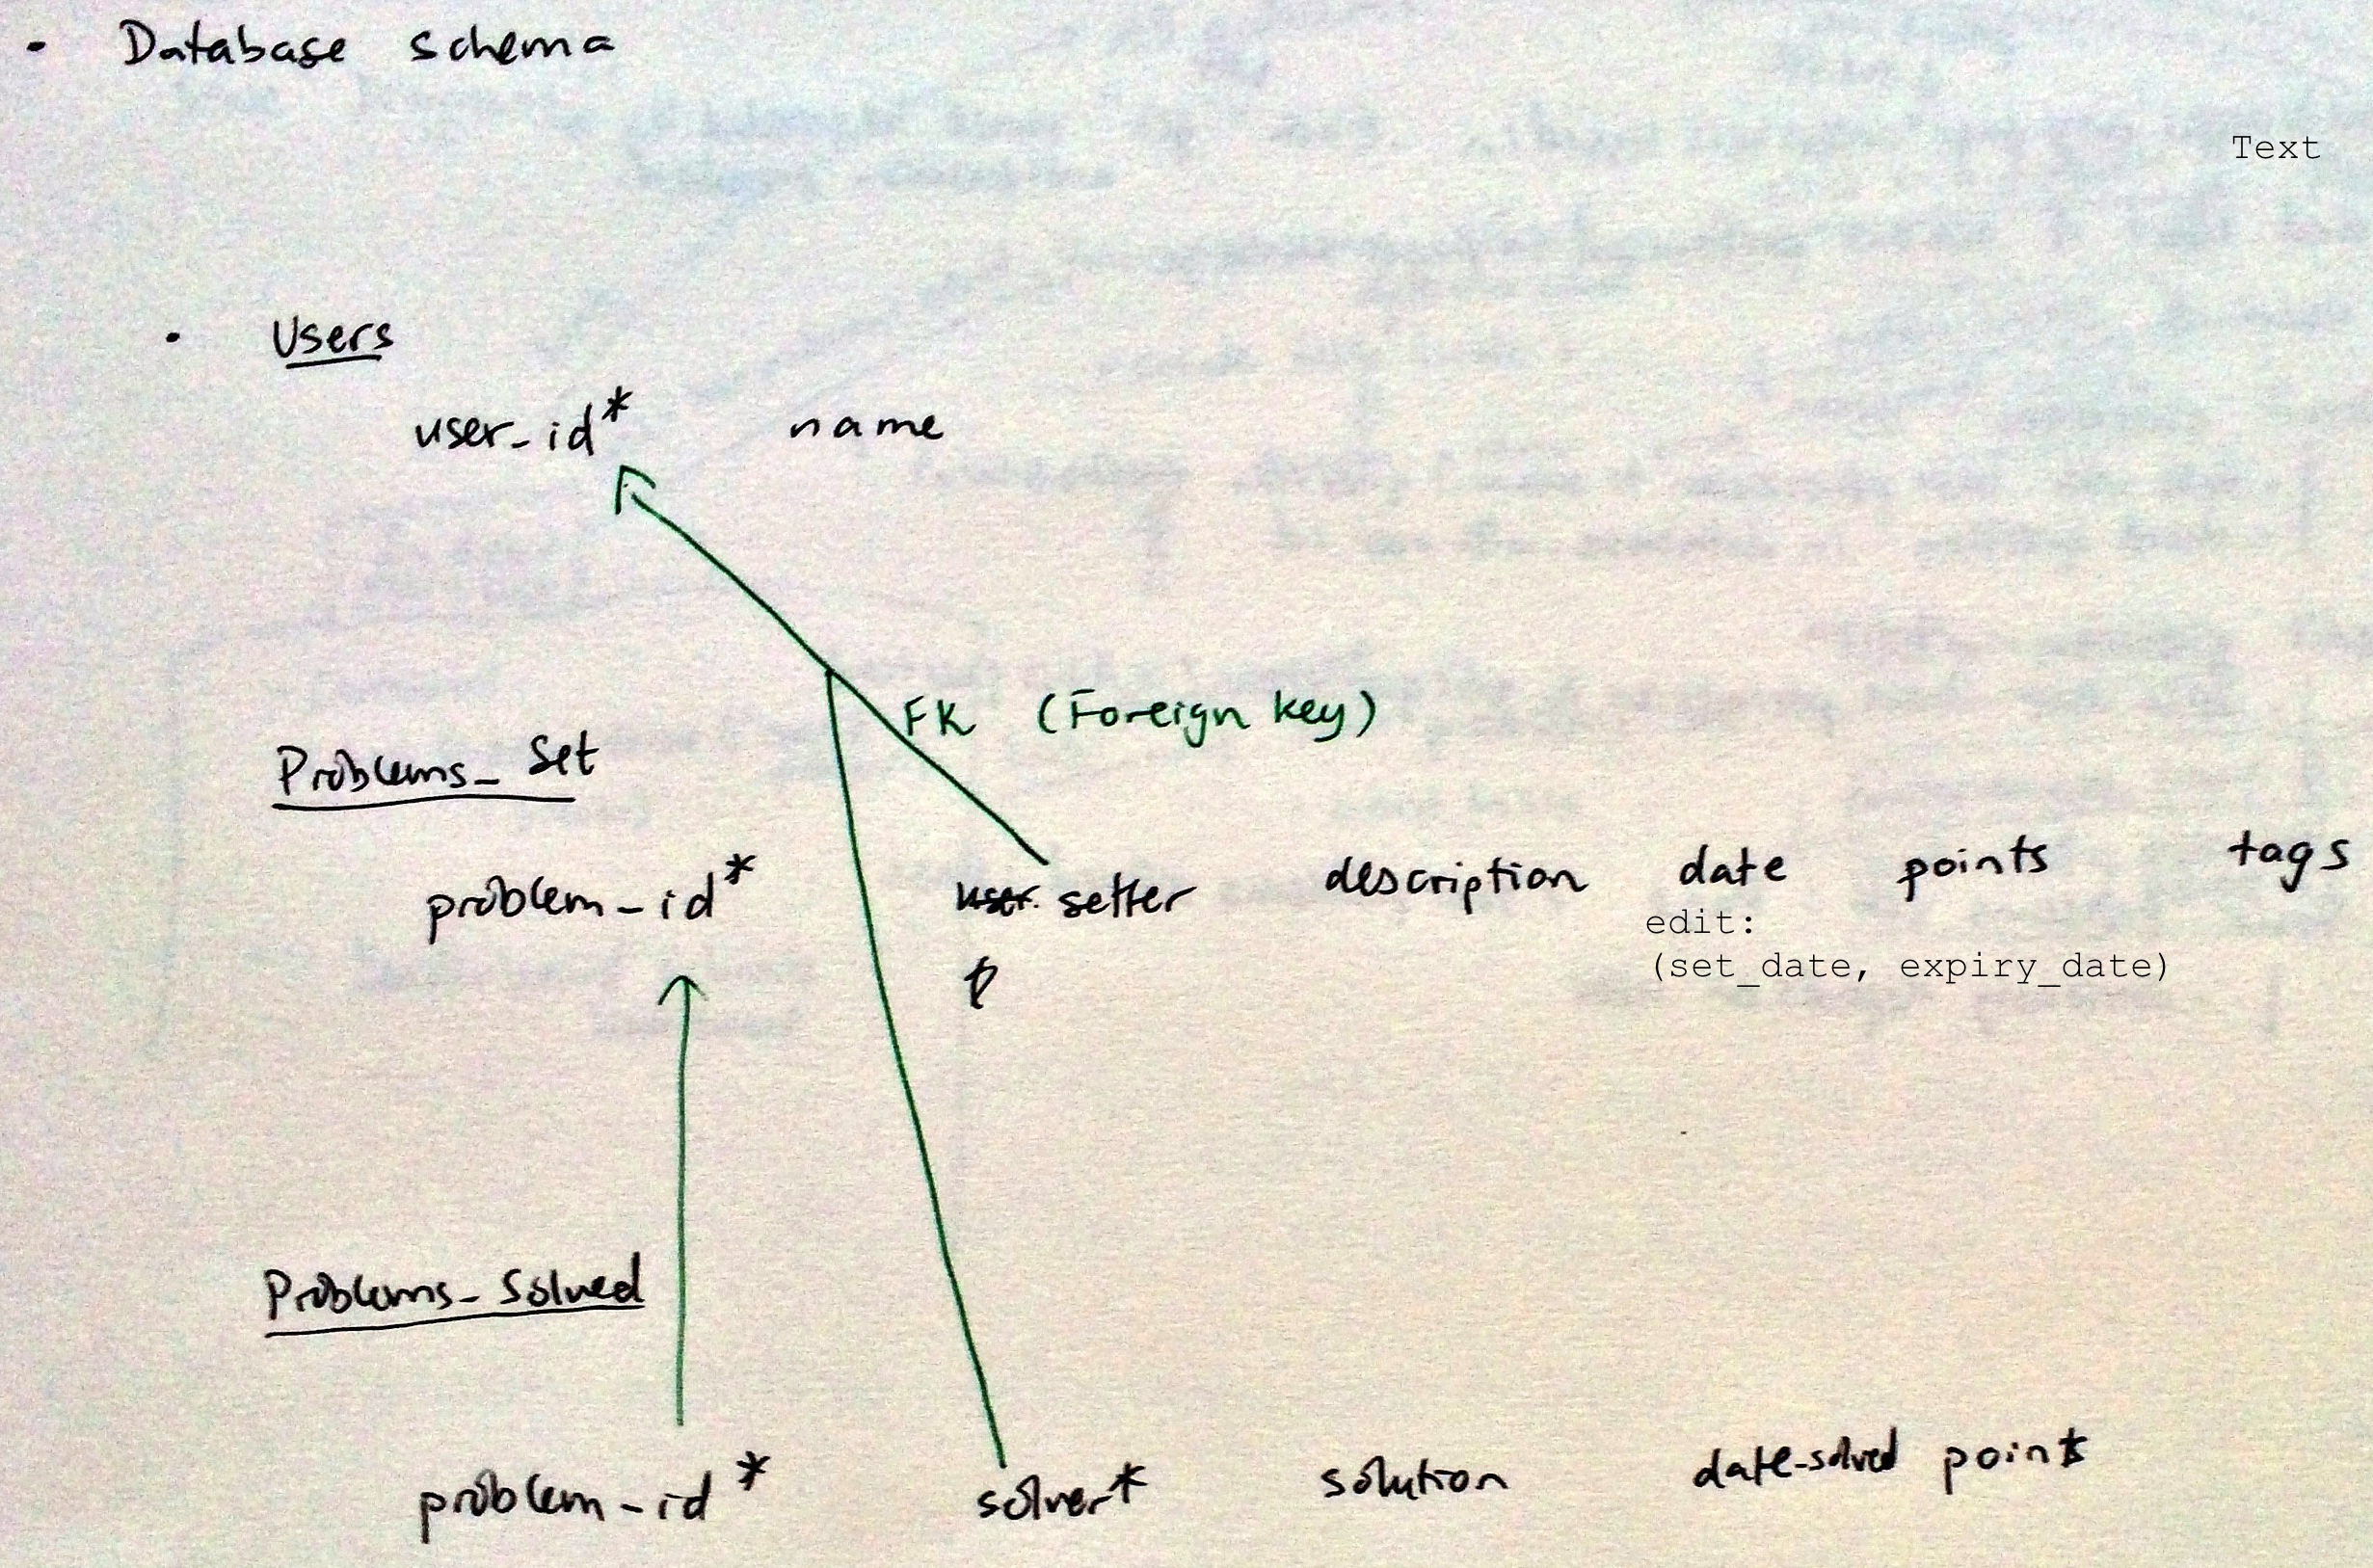
\includegraphics[width=\textwidth]{schema}
\caption{Database schema}
\end{figure}

\begin{figure}[H]
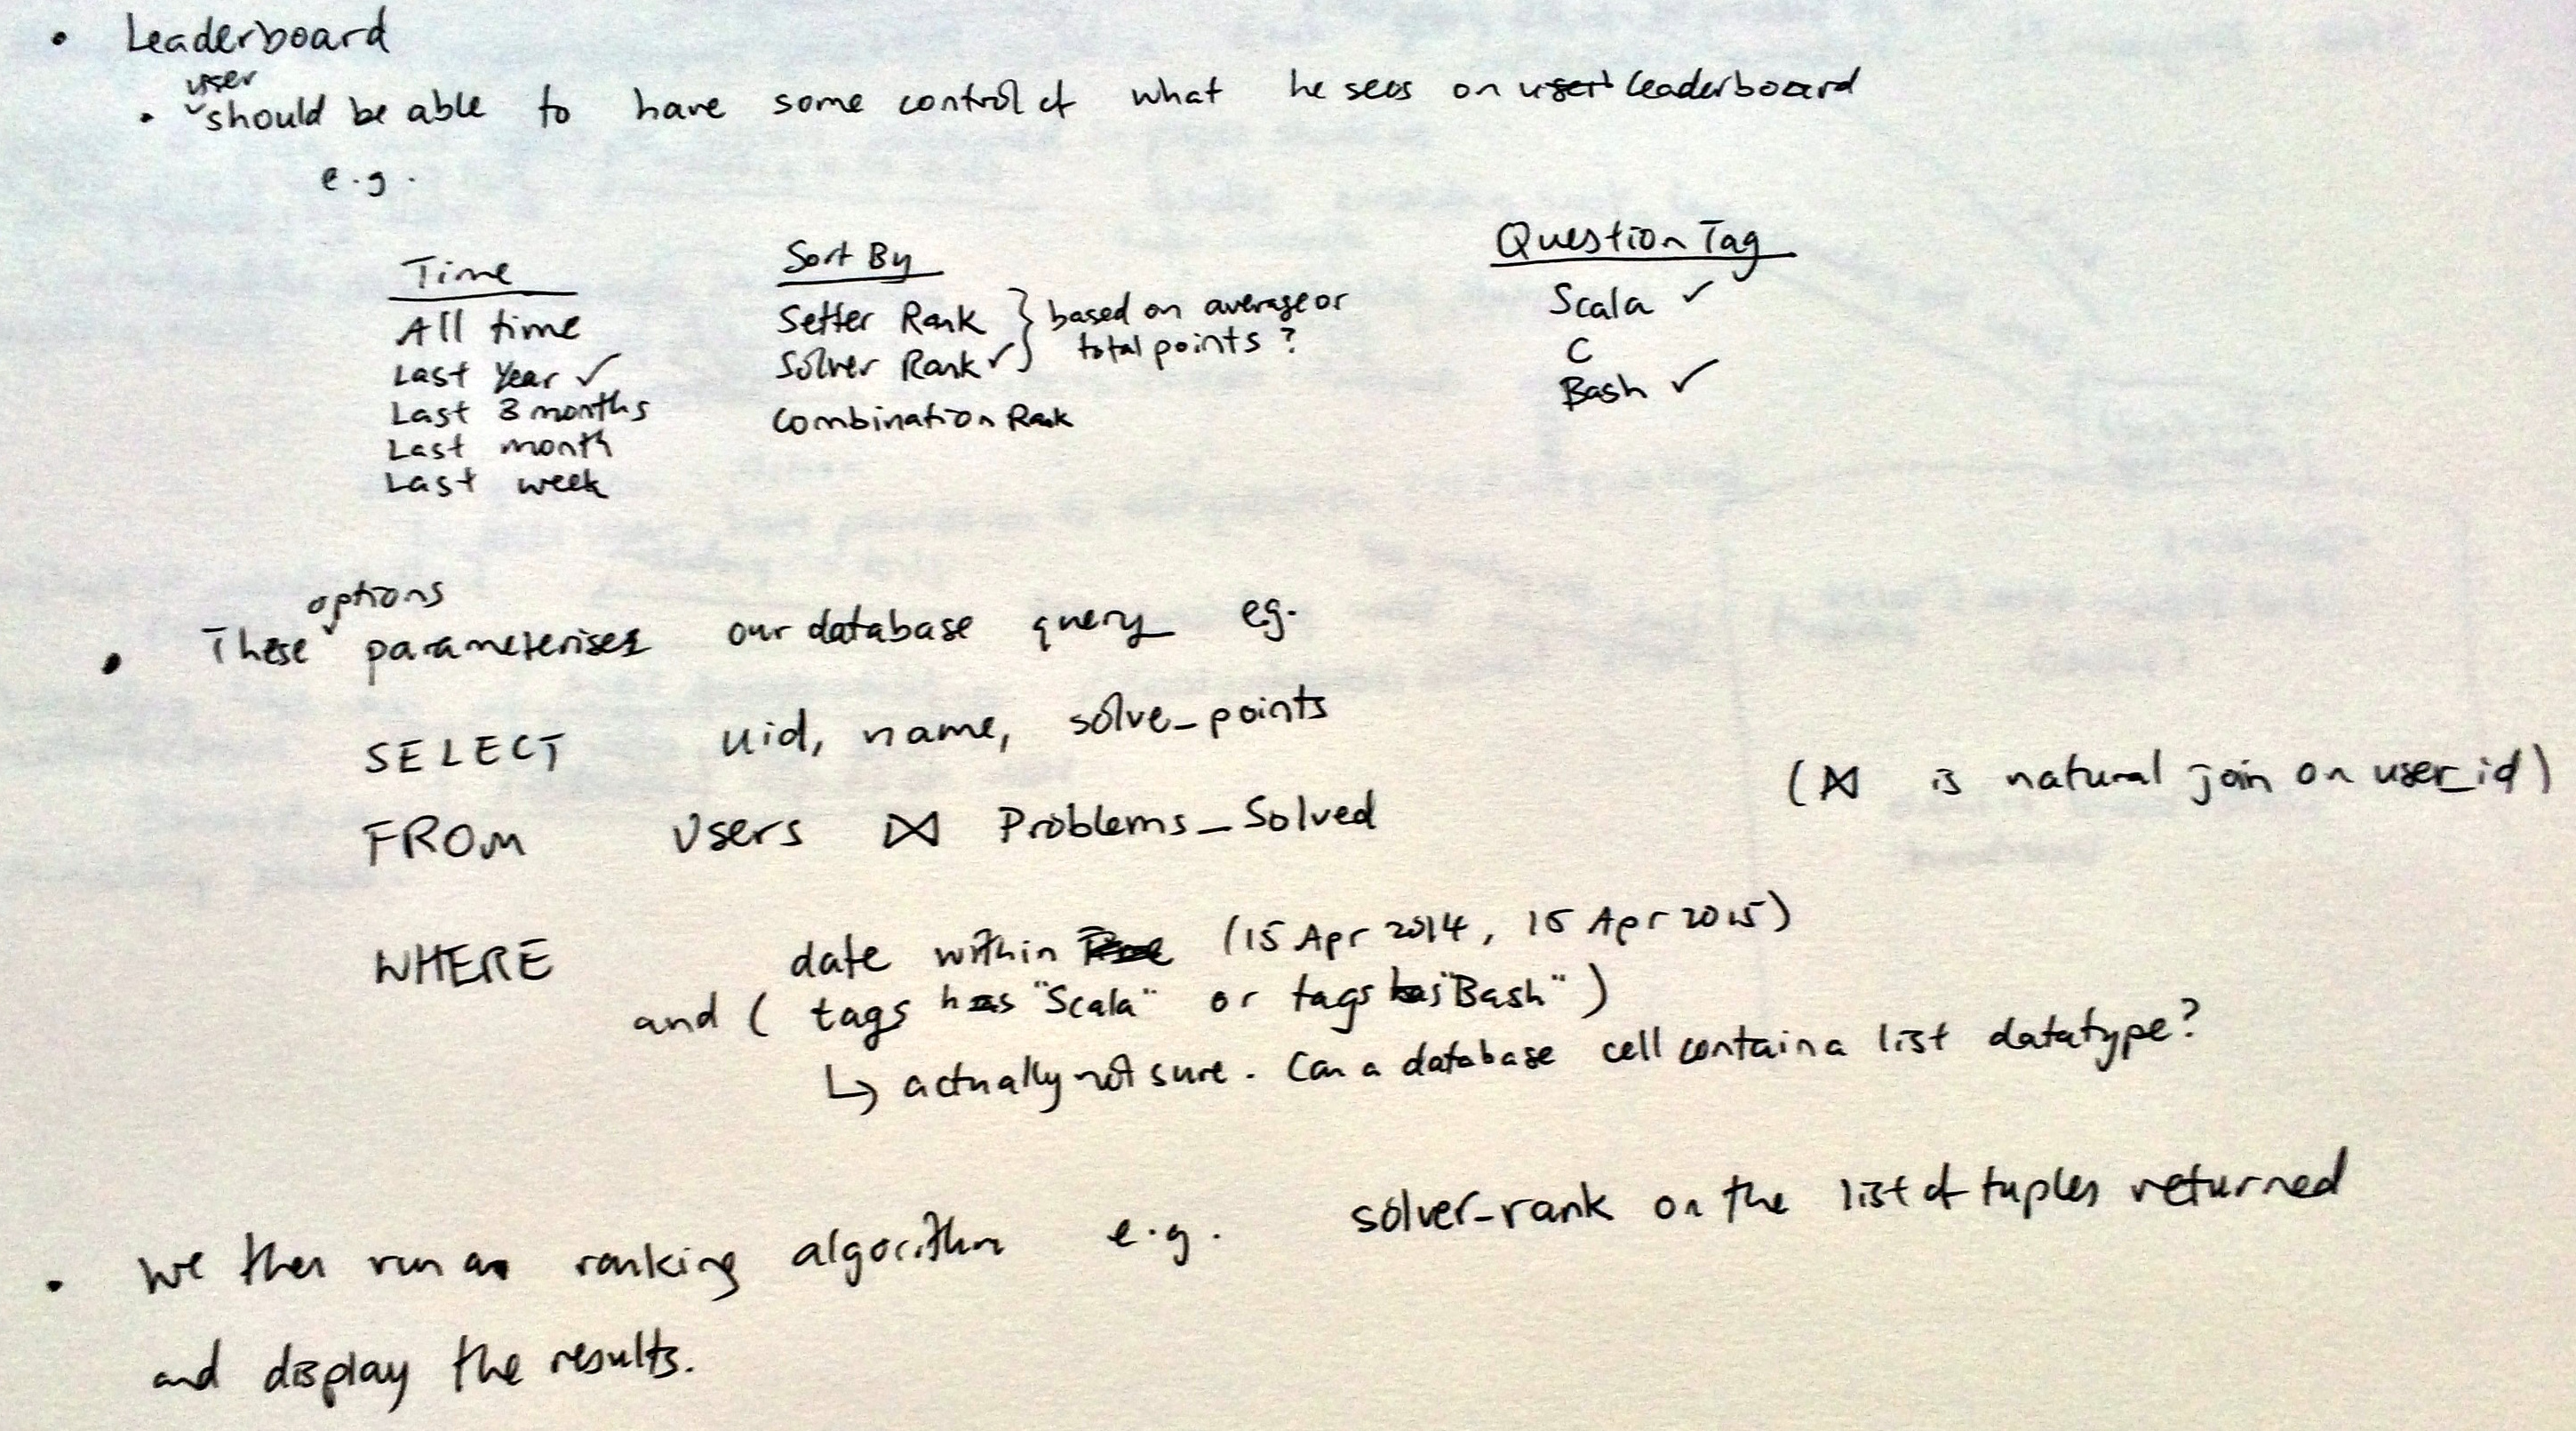
\includegraphics[width=\textwidth]{leaderboard}
\caption{Leaderboard functionality}
\end{figure}

\begin{figure}[H]
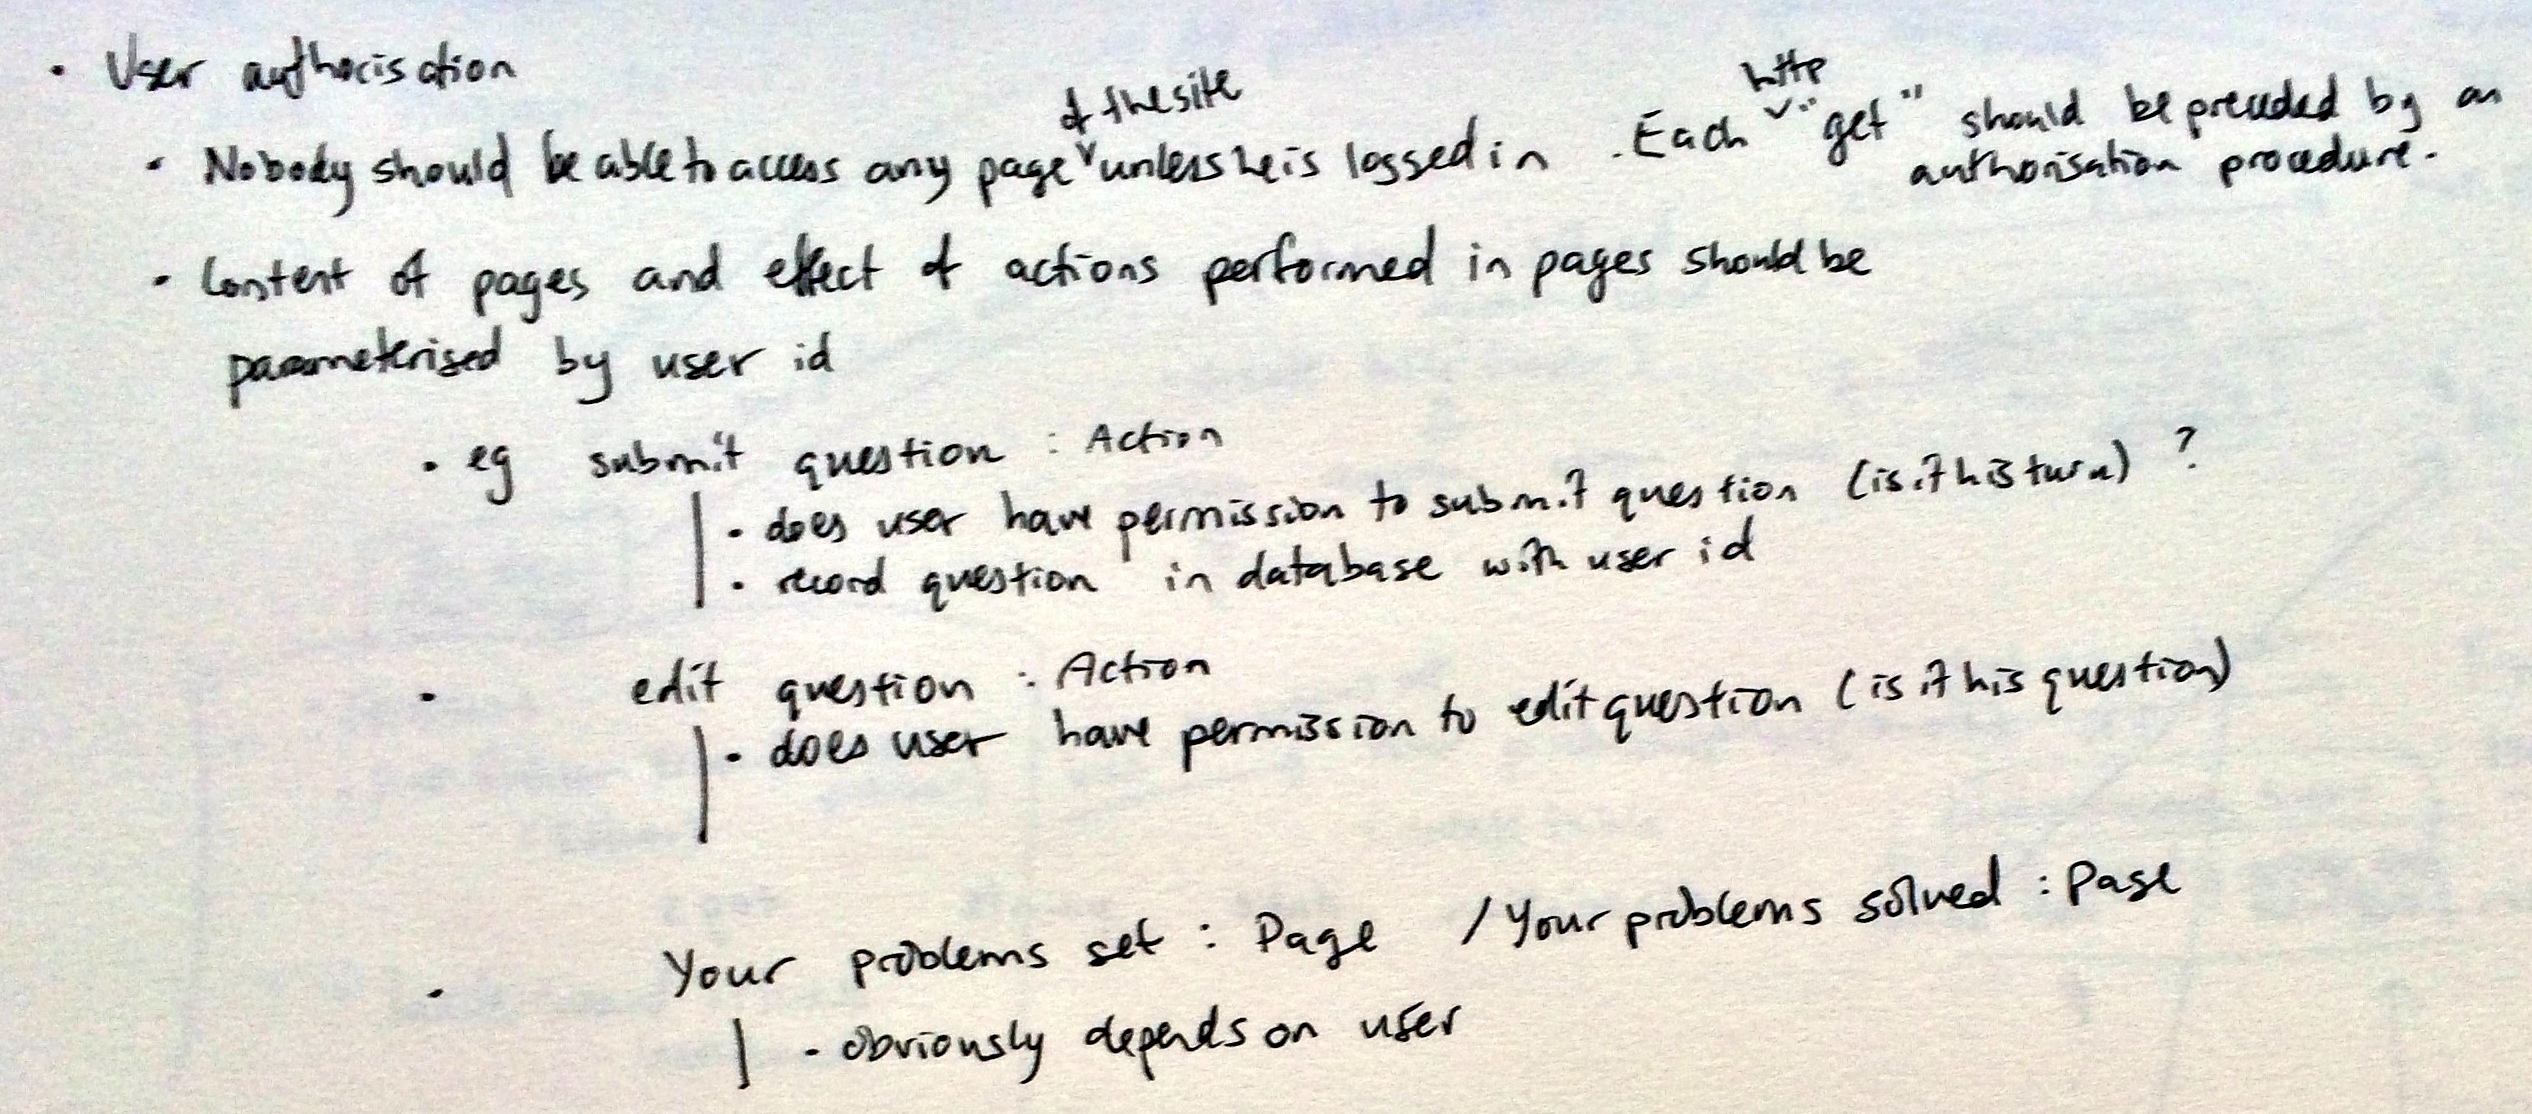
\includegraphics[width=\textwidth]{authorization}
\caption{User authorization}
\end{figure}

\section{States}
There are 4 main states. The application uses the methods outline in Figure 2.7 to decide which state it is in.

\begin{description}
  \item[Anyone is able to submit a challenge] \hfill \\ If there is no previous challenge then anyone can submit a challenge. This is the current state if \texttt{active\_problem?} is false and \texttt{most\_recent\_problem} is \texttt{nil}
  \item[The QM can set a challenge] \hfill \\ If the previous challenge has ended then the winner of that challenge can set the next challenge. This is the current state if \texttt{most\_recent\_problem.winner} is not \texttt{nil} and \texttt{active\_problem?} is false
  \item[The solvers can submit solutions] \hfill \\ If the QM has submitted a challenge and it has not ended yet, the solvers can all submit solutions. One solver can submit one solution. This is the state if \texttt{active\_problem?} is true.
  \item[The QM can grade the solutions] \hfill \\ When the challenge has ended the QM can grade the solutions. The challenge ends when either it expires (using the date given by the QM) or when all the solvers have submitted solutions. This is the state if \texttt{active\_problem?} is false and \texttt{most\_recent\_problem.winner} is \texttt{nil}
\end{description}

\begin{figure}[h]
\begin{verbatim}
module ProblemHelper
    def active_problem?
        ps = Problem.order(:created_at => :desc)
        if ps.size == 0 then false else ps.first.expiry > DateTime.now end
    end

    def most_recent_problem
        Problem.order(:created_at => :desc).first
    end
end
\end{verbatim}
\caption{The \texttt{ProblemHelper} class used to determine the app's state}
\end{figure}

\begin{figure}[H]
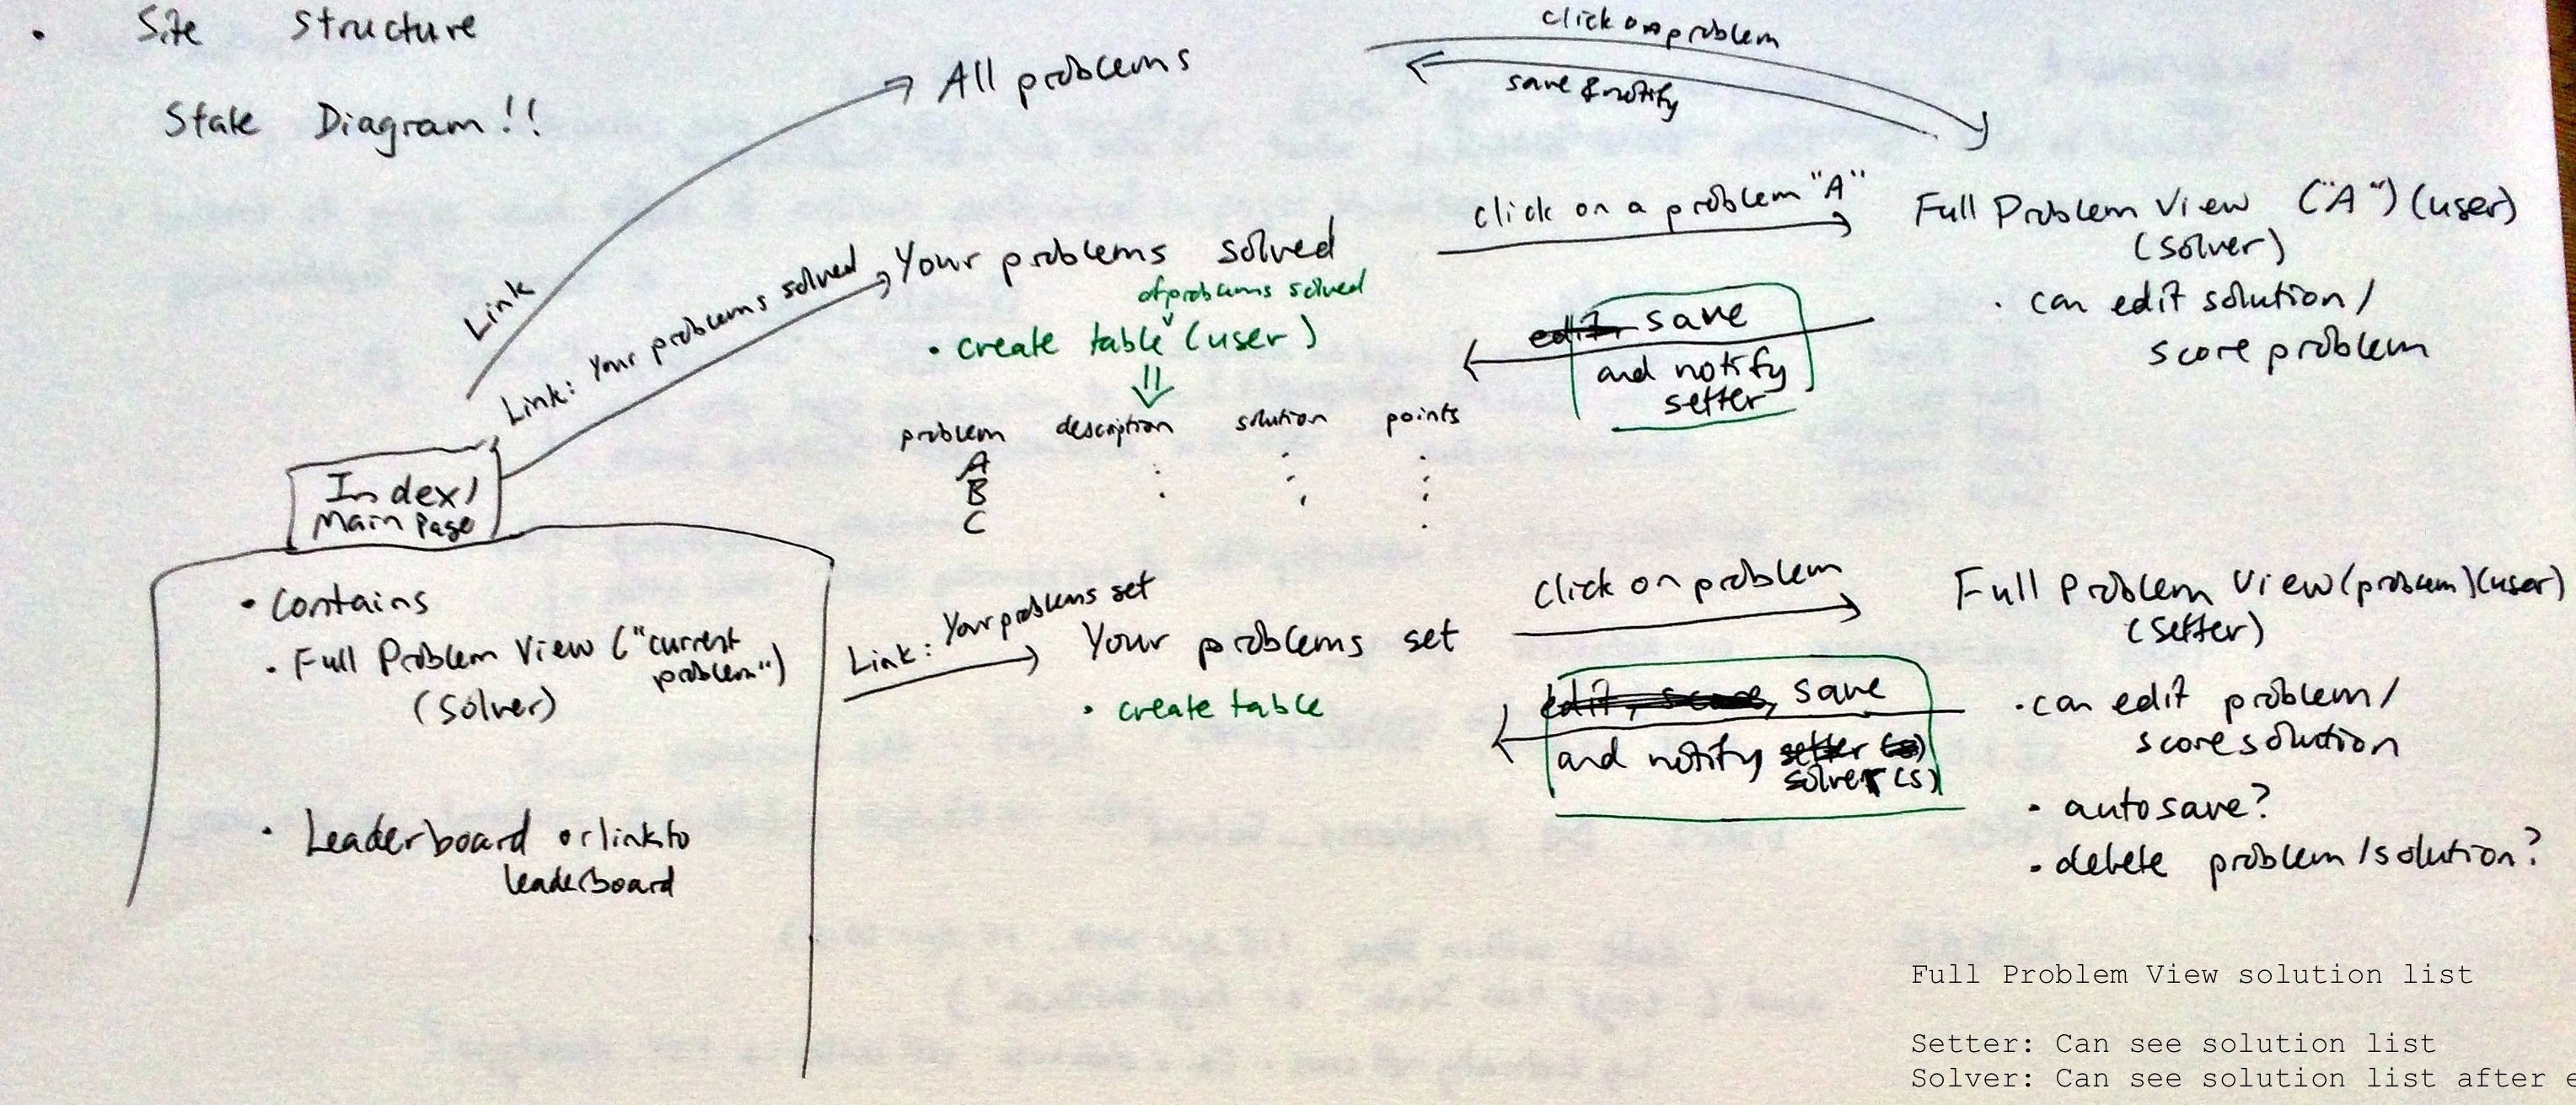
\includegraphics[width=\textwidth]{structure}
\caption{Proposed state diagram}
\end{figure}


\section{Back end design}
Initially we looked into using a \emph{Scala}-run server, but quickly we realised that the database library (\emph{Slick}) wasn’t well documented and the server itself would be very slow. Thus we changed to using \emph{Ruby on Rails} and \emph{SQLite}.

\emph{Rails} is incredibly powerful and versatile, but most importantly, it has been used for thousands and thousands of applications already. This means that there is a lot of documentation and support for common issues, as well as quick-start guides to help us get up and running in the short amount of time we had. Moreover, all of us were new to the \emph{Ruby} programming language and so were excited to try it out.

\section{Front end design}
Initially we tried building the website using a basic responsive framework \emph{Skeleton} (\url{http://getskeleton.com}) but soon realised that it would take too long to write the CSS for everything, so we moved to Twitter’s \emph{Bootstrap} (\url{http://getbootstrap.com}), which is more complete. We also are using \emph{FontAwesome} icons to improve usability.

As the website is built on a responsive framework, it is fully compatible to view on a mobile website, although the expectation is that users would likely use it from a computer as they can type out challenges and solutions more easily.


\section{Tests}
Throughout building the application we have been testing with sample problems and solutions to get everything working. When it was complete, we allowed seven real-world (non-CS!) testers onto our server to try it out, and were given feedback praising the design and its ease-of-use. A few bugs (regarding mobile website sizing and a link on the FAQ page) were also squashed.

\section{Extensions}
One extension that would help would be to create individual domains for different companies or groups to use, in the same way that \emph{Slack} does. This would allow more specialised questions for the companies using them.

We have a template in place on the dashboard where awards would go, but have not implemented them. Awards for a coding challenge would for example be `Best Comments`, `Most Concise Code`, etc. Implementing an awards system would help by increasing competition between users.

\appendix

\chapter{Desktop screenshots}
Chrome 42.0.2311\\Microsoft Windows 8\\\url{http://robin.robertbastian.de}

\begin{figure}
\fbox{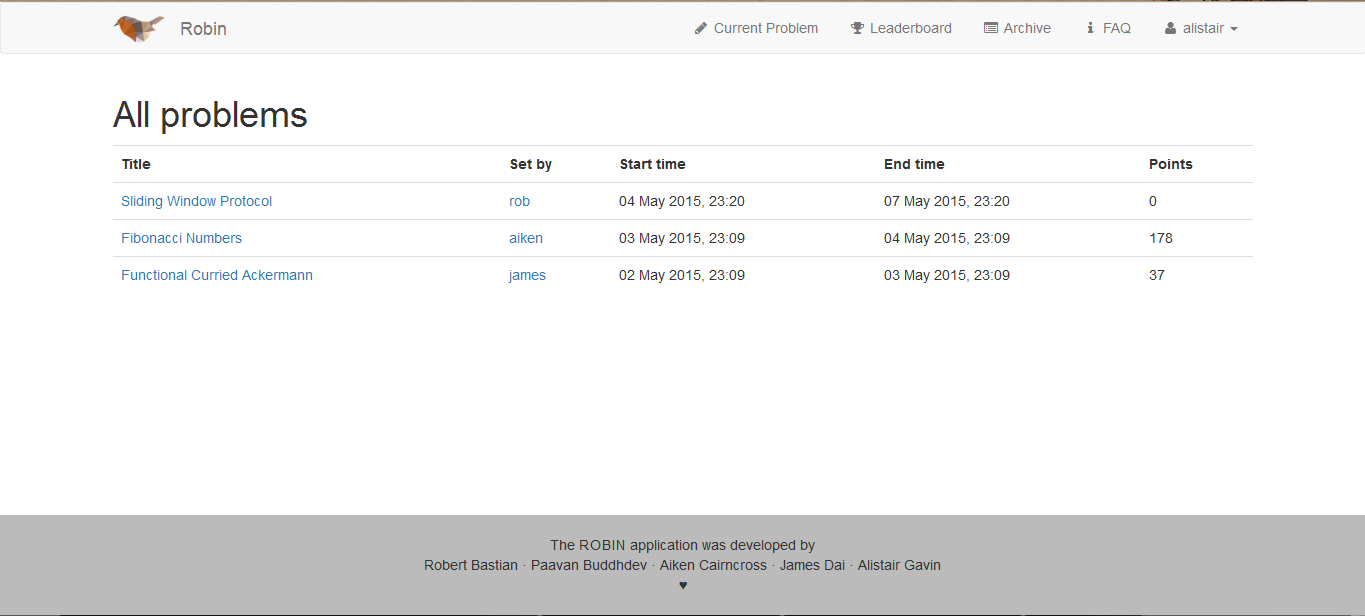
\includegraphics[width=\textwidth]{Archive}}
\caption{Archive}
\end{figure}

\begin{figure}
\fbox{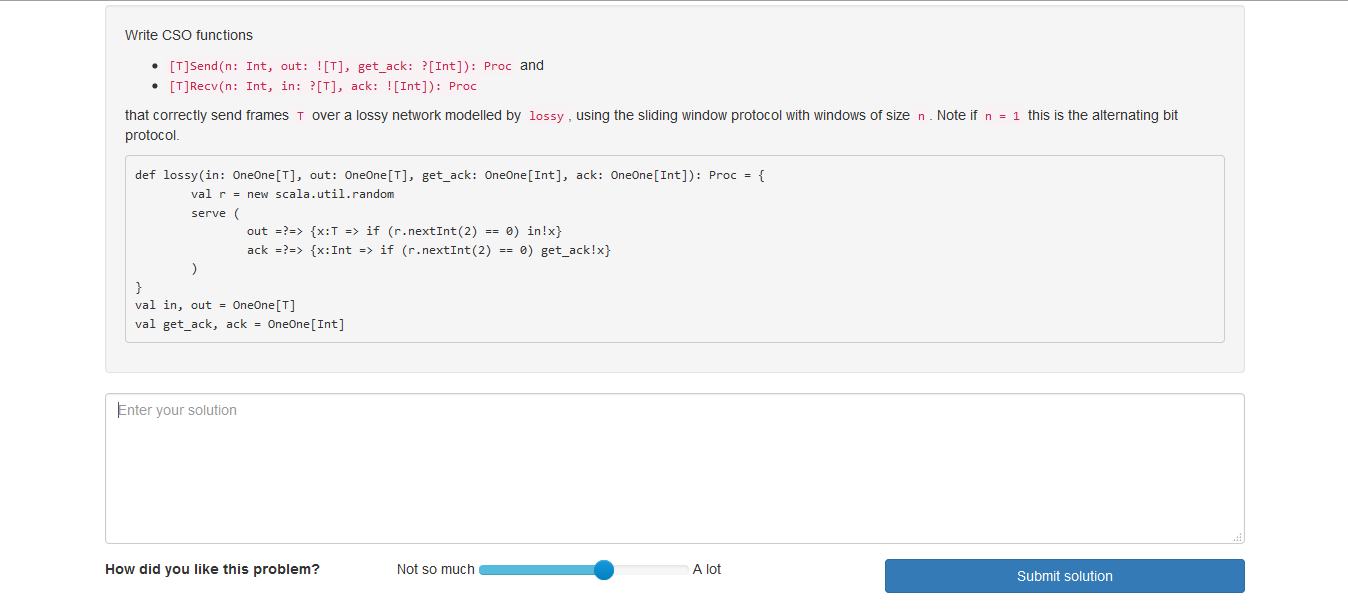
\includegraphics[width=\textwidth]{CreateSolution}}
\caption{Solution creation page}
\end{figure}

\begin{figure}
\fbox{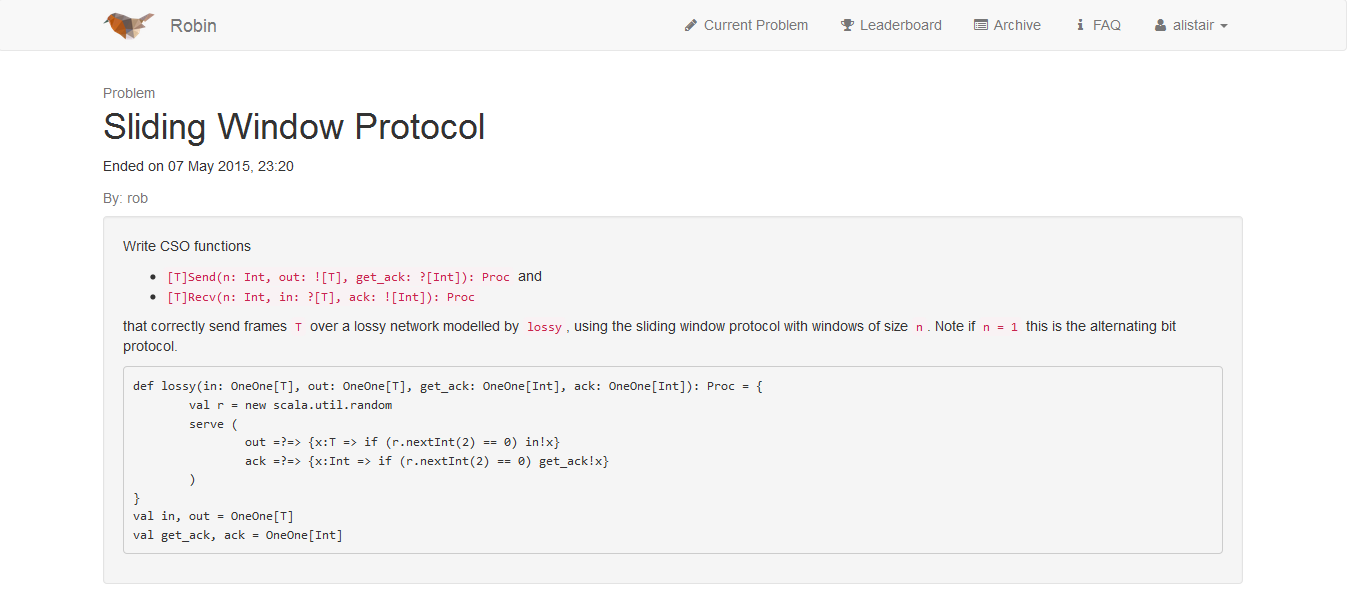
\includegraphics[width=\textwidth]{CurrentProblem}}
\caption{Current problem}
\end{figure}

\begin{figure}
\fbox{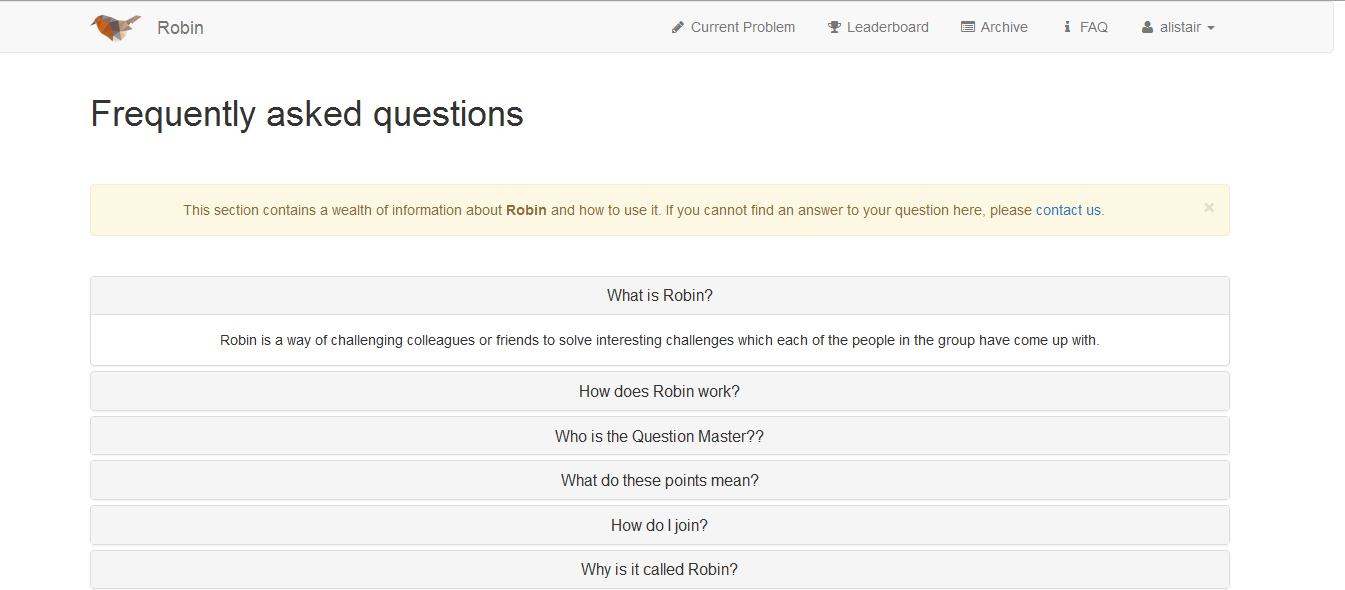
\includegraphics[width=\textwidth]{FAQ}}
\caption{Frequently asked questions}
\end{figure}

\begin{figure}
\fbox{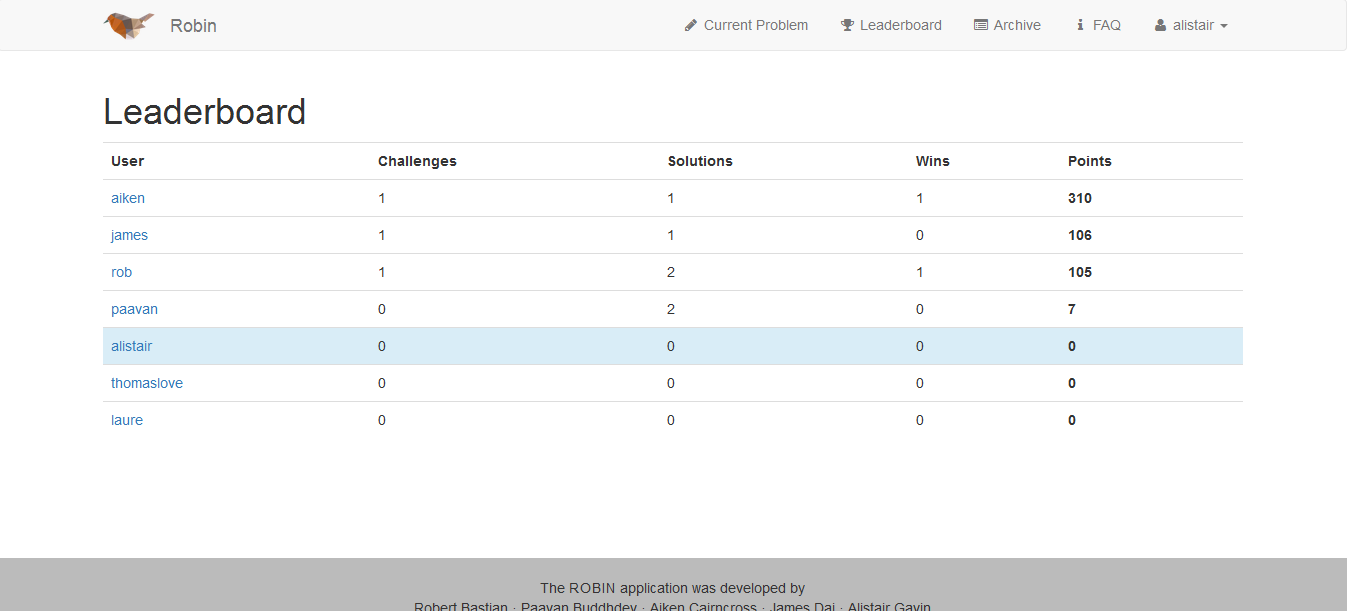
\includegraphics[width=\textwidth]{Leaderboard}}
\caption{Leaderboard}
\end{figure}

\begin{figure}
\fbox{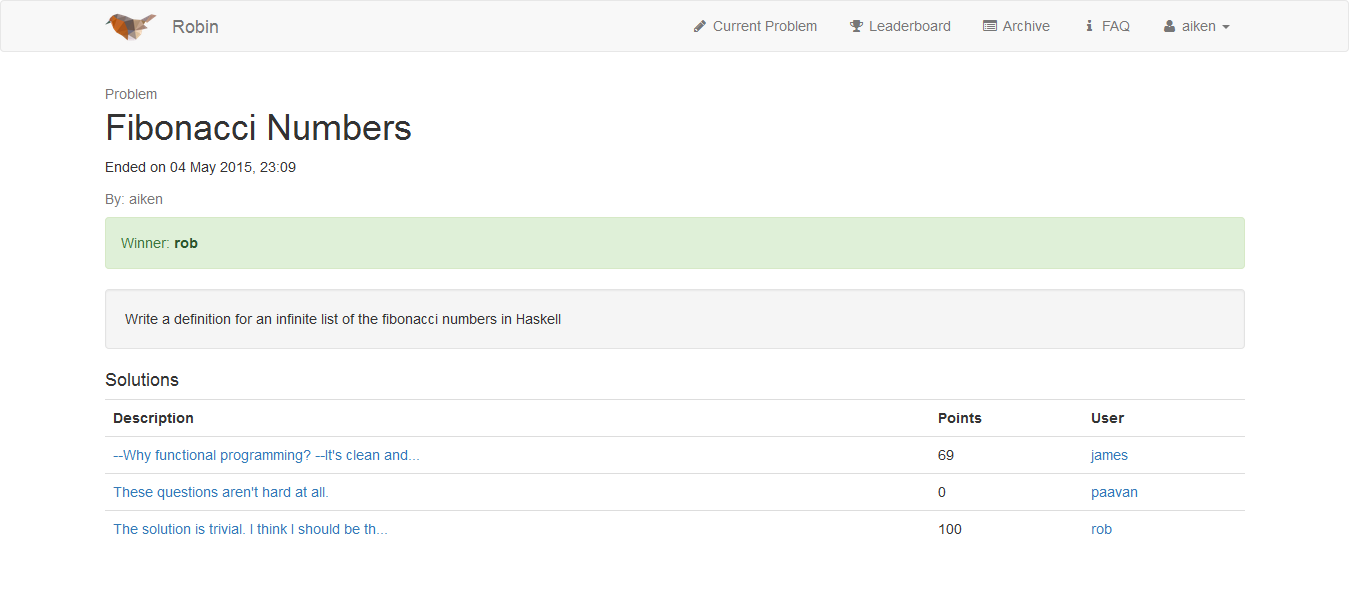
\includegraphics[width=\textwidth]{ProblemExample}}
\caption{Finished challenge}
\end{figure}

\begin{figure}
\fbox{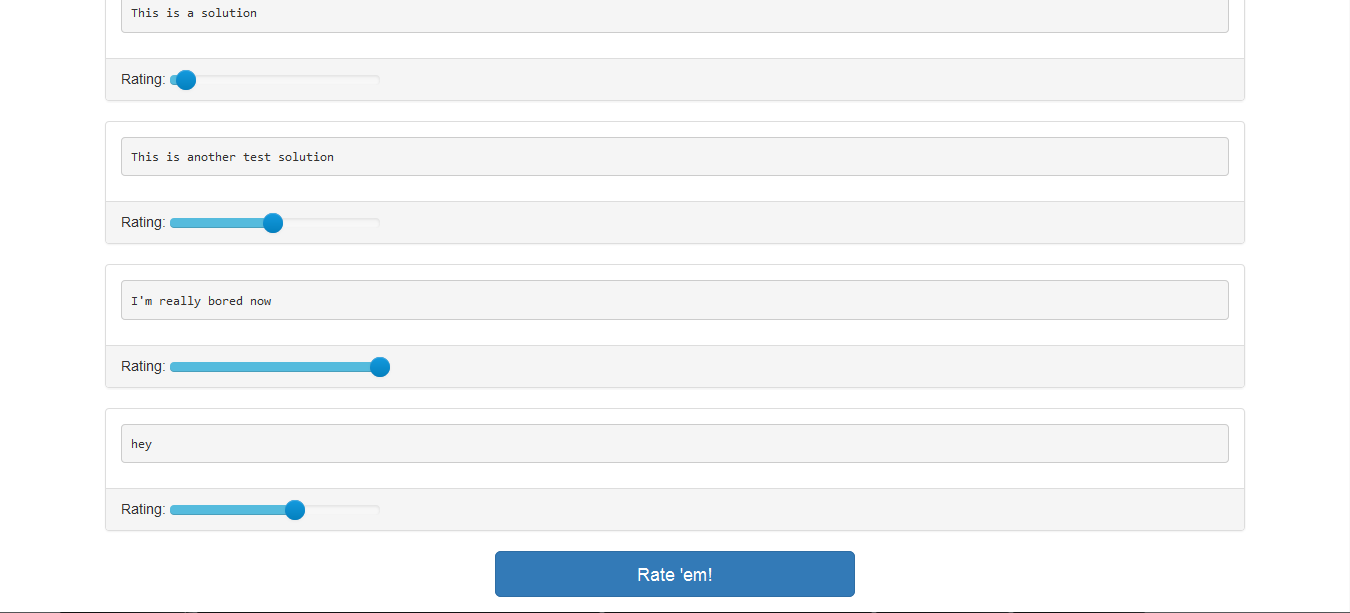
\includegraphics[width=\textwidth]{ProblemMarking}}
\caption{Challenge marking}
\end{figure}

\begin{figure}
\fbox{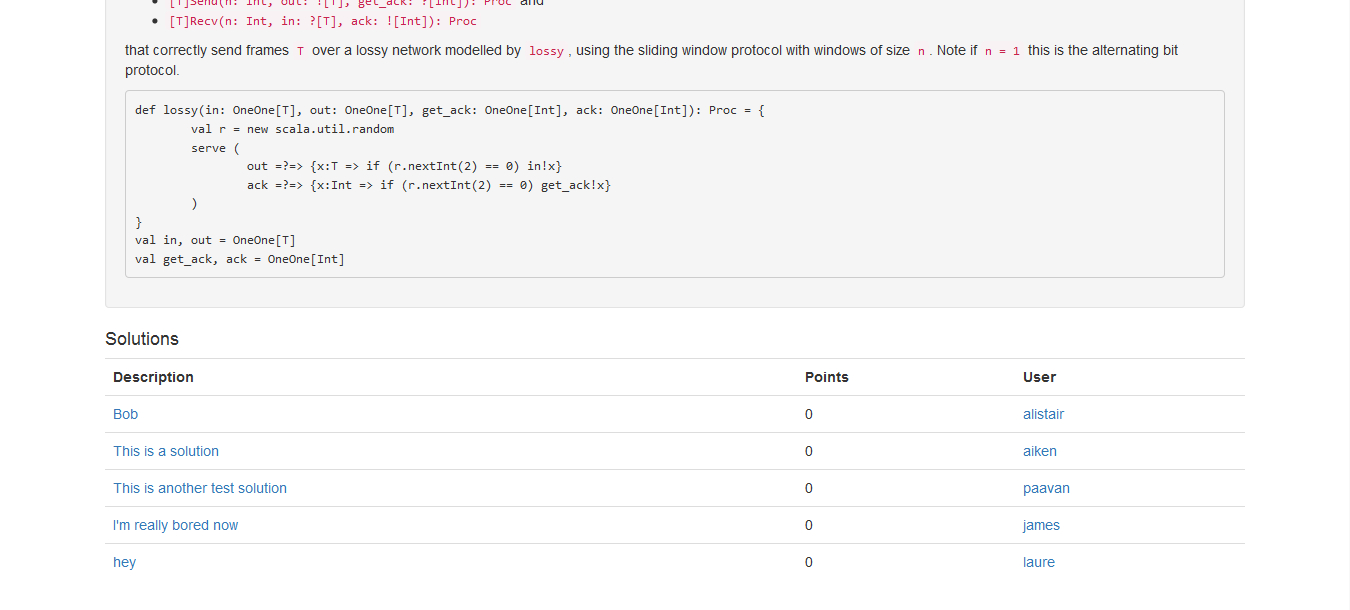
\includegraphics[width=\textwidth]{ProblemSubmitterView}}
\caption{Question Master's view of a challenge}
\end{figure}

\begin{figure}
\fbox{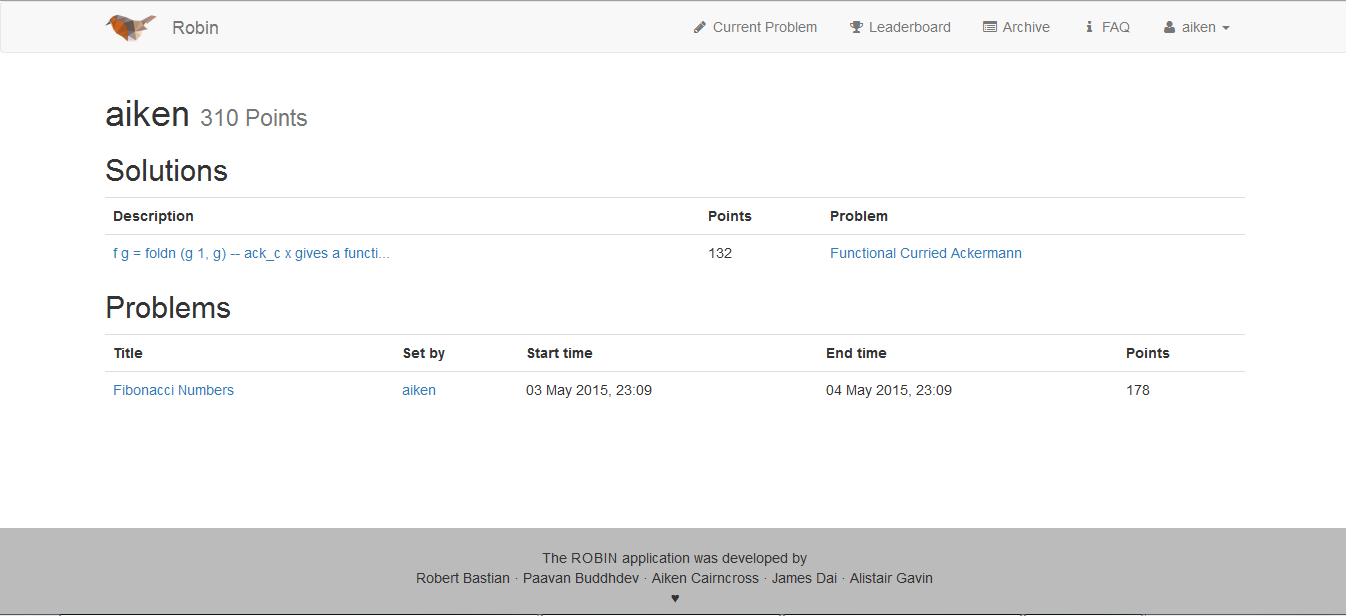
\includegraphics[width=\textwidth]{Profile}}
\caption{Profile}
\end{figure}

\begin{figure}
\fbox{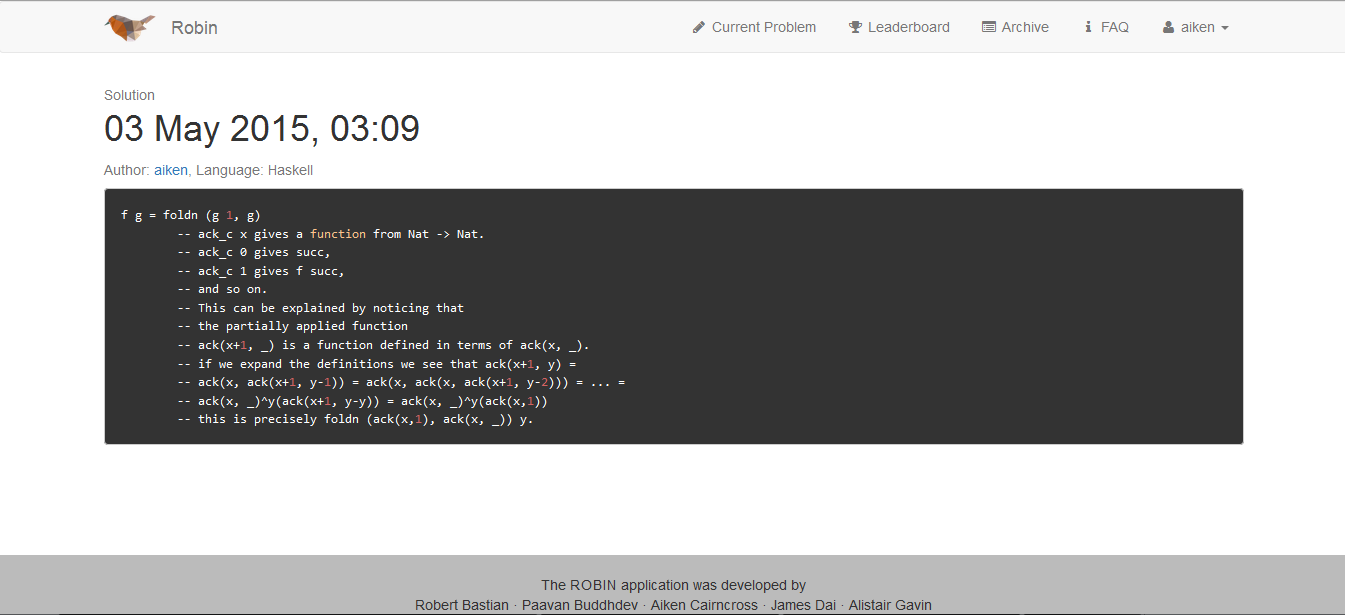
\includegraphics[width=\textwidth]{Solution}}
\caption{Solution}
\end{figure}

\chapter{Mobile screenshots}
Chrome 42.0.2311.47\\iOS 8/iPhone 5\\\url{http://robin.robertbastian.de}

\begin{figure}
\fbox{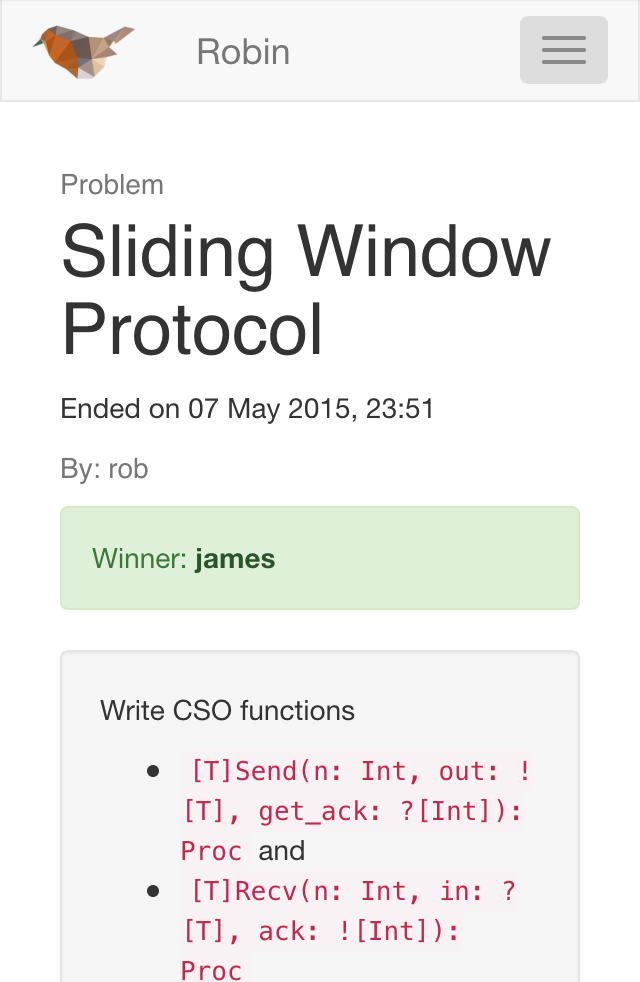
\includegraphics[width=\textwidth]{IMG_0798}}
\caption{Problem page}
\end{figure}

\begin{figure}
\fbox{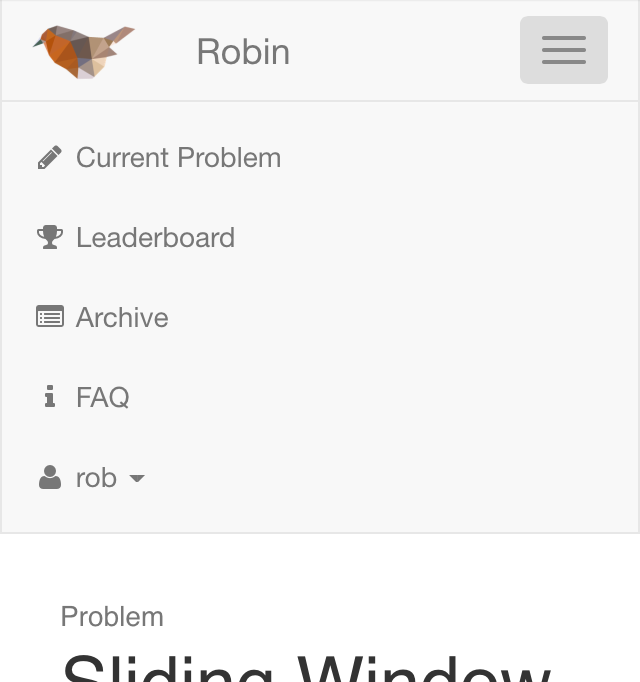
\includegraphics[width=\textwidth]{IMG_0799}}
\caption{Menu}
\end{figure}

\begin{figure}
\fbox{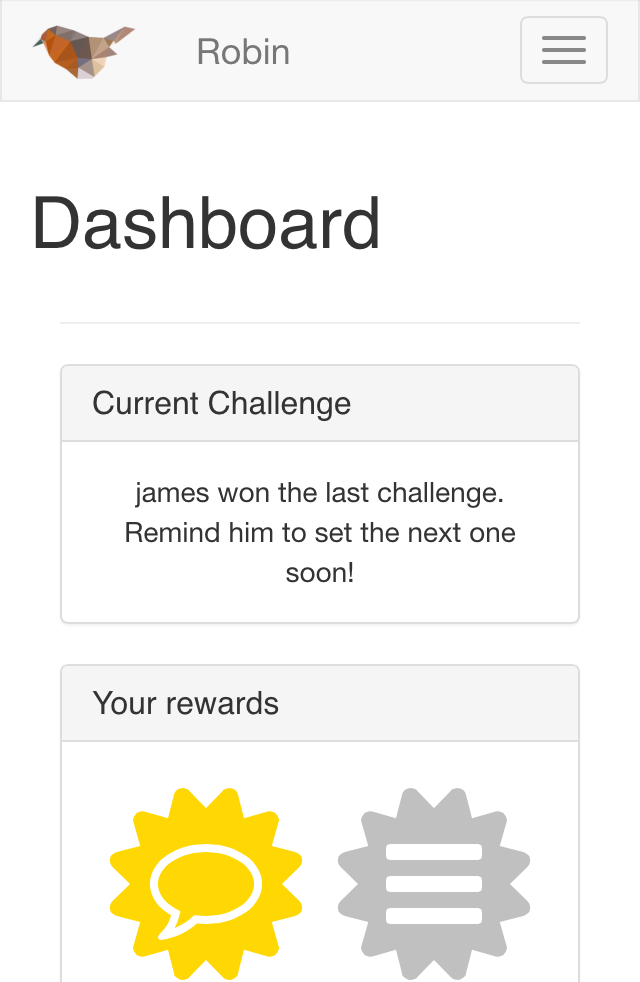
\includegraphics[width=\textwidth]{IMG_0800}}
\caption{Dashboard}
\end{figure}

\begin{figure}
\fbox{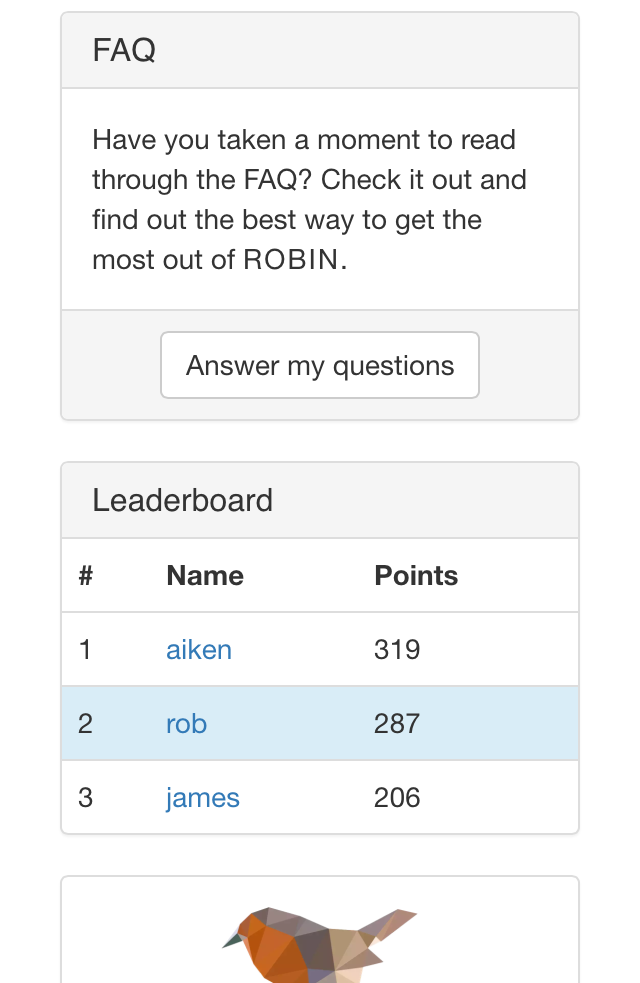
\includegraphics[width=\textwidth]{IMG_0802}}
\caption{Dashboard with leaderboard}
\end{figure}

\begin{figure}
\fbox{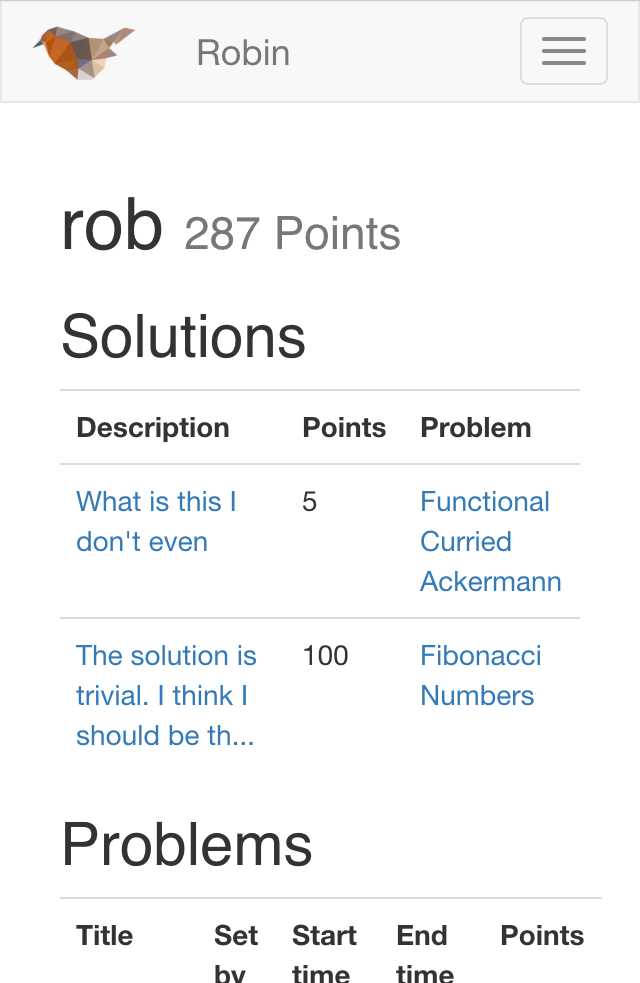
\includegraphics[width=\textwidth]{IMG_0801}}
\caption{User page}
\end{figure}

\end{document}
